\documentclass{beamer}
\mode<presentation>
\usepackage{amsmath}
\usepackage{amssymb}
%\usepackage{advdate}
\usepackage{graphicx}
\graphicspath{{../figs/}}
\usepackage{adjustbox}
\usepackage{subcaption}
\usepackage{enumitem}
\usepackage{multicol}
\usepackage{mathtools}
\usepackage{listings}
\usepackage{url}
\def\UrlBreaks{\do\/\do-}
\usetheme{Boadilla}
\usecolortheme{lily}
\setbeamertemplate{footline}
{
  \leavevmode%
  \hbox{%
  \begin{beamercolorbox}[wd=\paperwidth,ht=2.25ex,dp=1ex,right]{author in head/foot}%
    \insertframenumber{} / \inserttotalframenumber\hspace*{2ex} 
  \end{beamercolorbox}}%
  \vskip0pt%
}
\setbeamertemplate{navigation symbols}{}


\lstset{
%language=C,
frame=single, 
breaklines=true,
columns=fullflexible
}
\let\solution\relax
\usepackage{gvv}
\numberwithin{equation}{section}
\title{4.7.62}
\author{AI25BTECH11001 - ABHISEK MOHAPATRA}
% \maketitle
% \newpage
% \bigskip
\begin{document}
{\let\newpage\relax\maketitle}
\renewcommand{\thefigure}{\theenumi}
\renewcommand{\thetable}{\theenumi}


	 	\textbf{Question}:
Find the equation of the plane which passes through the point (5,2,-4) and perpendicular the line with direction ratios 2,3,-1.


		\textbf{Solution:} let the equation of the plane be 
\begin{align}
		\vec{n}^\top\vec{x} = c
\end{align}

as per the question, $\vec{n} = \myvec{2\\3\\-1}$ and a point ,let $\vec{P} = \myvec{5\\2\\-4}$ 

so putting the values in the equation,
\begin{align}
		\myvec{2\\3\\-1}^\top\myvec{5\\2\\-4} = c\\
		\Rightarrow c = 10 + 6 +4 = 20
\end{align}
so the required equation is
\begin{align}
		\myvec{2&3&-1}\vec{x} = 20
\end{align}

Graph:
\begin{figure}[h!]
	\centering
	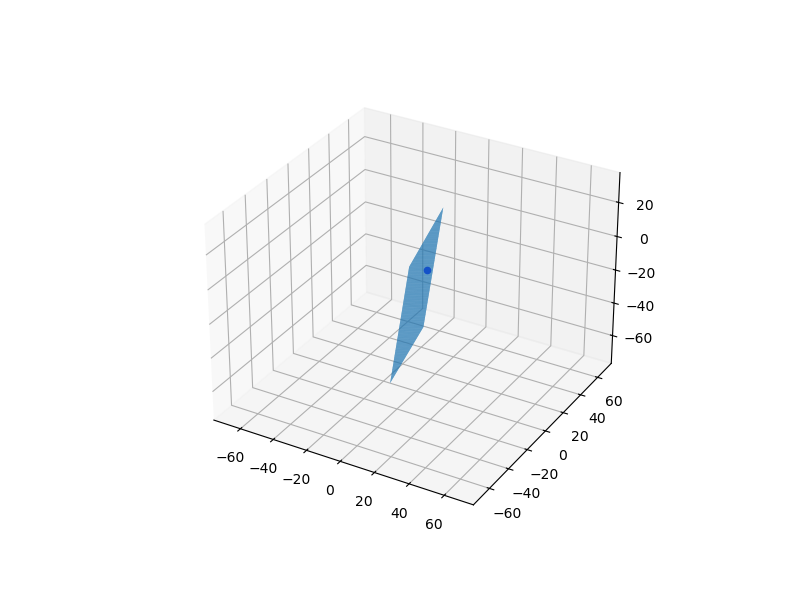
\includegraphics[width=0.7\linewidth]{img.png}
\end{figure}
\end{document}


